\section{Practical Aspects} \label{sec:practical_aspects}

We address here some issues that arise when implementing the described algorithm on a resource-constrained platform. Furthermore, we introduce many practical expedients that deal with limited sampling budget, slow control rates and finally with sim-to-real transfer.  

\subsection{Gradient Clipping} 
The policy update rule in \eqref{eq:update_rule} consists of a receding horizon \emph{mini-batch} SGD. As a consequence, the gradient variance can vary greatly between successive iterations of the algorithm. To prevent this phenomenon, which is especially evident with a small sampling budget, we clip the gradients to a user-defined threshold.  

\subsection{Likelihood mapping} 
The coefficient $\lambda$ in \eqref{eq:weighting} determines how much ``aggressive" the weighting between different trajectories is. Adopting a constant value would give a numerically zero weight to most of the trajectories. Shifting the trajectory cost by the minimum cost as proposed in~\cite{williams_information_2017} also does not alleviate this issue. 
Especially in regions of high cost, trajectories that are equivalently good can be assigned very different weights. We instead propose to adopt the same technique as in~\cite{theodorou2010generalized} where the $\lambda$ is scaled to better discriminate between the experienced trajectories. The modified exponential utility is then defined by,
\begin{equation} \label{eq:scale_invariant_mapping}
    \exp (-\lambda J ) = \exp \left( -h \frac{J - J_{\min}}{J_{\max} - J_{\min}} \right).
\end{equation}
which has the nice property of being invariant to the cost scale. Assume for example, that in a target reaching task, the goal pose is far away and thus the cost incurred by each sampled rollout is scaled by a common scalar factor. This factor would disappear when using the previous equation for mapping rollouts to likelihood. We show the effect of cost-scale invariance in \fig \ref{fig:exponential_mapping_comparison}. In the figure we assume that samples' costs are uniformly distributed in the range between minimum and maximum cost and that the minimum cost shows a $20$\% reduction with respect to the worse rollout\footnote{This is a reasonable choice since we are in a online setup and we assume to be in a low sampling budget regime.}. We compare the exponential mapping $\mathcal{J} = \exp(-\lambda J)$ (\textit{naive}), with baseline reduction $\mathcal{J} = \exp(-\lambda (J - J_{min}))$ (\textit{baseline}) and the mapping in \eqref{eq:scale_invariant_mapping} (\textit{invariant}).

\begin{figure}[t]
    \centering
    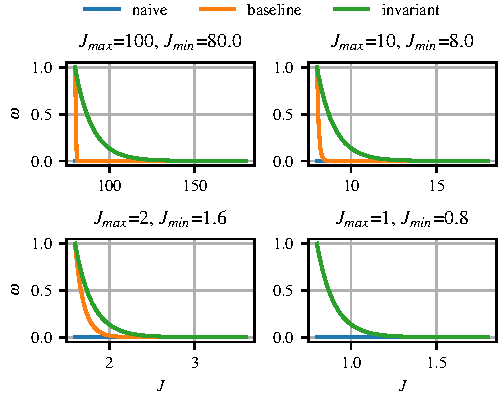
\includegraphics{figures/likelihood_mapping.pdf}
    \caption{In each plot we change the maximum and minimum cost ($80$\% of maximum cost). We set $\lambda$ and $h$ to 10 in all comparison.}
    \label{fig:exponential_mapping_comparison}
\end{figure}

When the cost is high, the first two methods collapse all the weight to a single sample and in practice, other samples are assigned a value which is numerically zero. As a consequence, the gradient estimate in \eqref{eq:update_rule} can show a high variance. The mapping in \eqref{eq:invariant_mapping} instead, assigns a non-zero weight to more samples independently from the current cost scale and helps to stabilize the gradient estimate.

\subsection{Chattering}
We observed that a naive implementation of the passivity constraint leads to a chattering behavior at the constraint boundary. We start discretizing the constraint inequality to obtain a constraint which is affine in the input $\command$:
\begin{equation*}
    \int_{0}^{t + dt} \boldsymbol{\tau}_{ext}^T \command \ dt \approx \underbrace{\boldsymbol{\tau}_{ext}(t)^T \command(t) dt}_{-P_{diss}} + S(x_t(t)) \geq \epsilon,
\end{equation*}
which is equivalent to 
\begin{equation} \label{eq:passivity_simple}
    P_{diss} \leq \alpha E_{res},
\end{equation}
where we defined the residual energy $S(x_t(t))-\epsilon$ as $E_{res}$. The above inequality has the drawback that when the Euler integration is performed with small time intervals, then a dangerously high power can be dissipated at any time, until very close to the lower energy limit, thus leading to chattering. It is therefore better to use a value of $\alpha < 1/dt$. Furthermore, one can easily verify that defining a passivity ZBF as $h_{pass} = S(x_t) - \epsilon$ we obtain the same formulation. The ZBF constraint reads as:
\begin{equation*}
    \dot{h}_{pass} = \dot{S}(x_t) \geq -\alpha h_{pass}
     =\alpha (\epsilon - S(x_t))).
\end{equation*}
The passivity can therefore seen as a ZBF and consequently inherits its properties. A smaller value for $\alpha$ makes the constraint more conservative and improves its performance at the boundary. In the worst case scenario, the dissipated power is always equal to the maximal power allowed by the passivity constraint: $\dot{E}_{res} = - \alpha E_{res}$. Then $E_{res}(t) = E_{res}(0) e^{-\alpha t}$. A smaller $\alpha$ makes the energy drop more slowly and avoids a fast depletion of the tank as shown in \fig \ref{fig:worst_case_energy_profile}.
\begin{figure}[t]
    \centering
    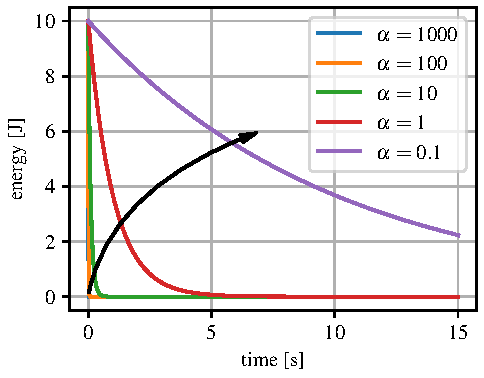
\includegraphics[width=0.8\columnwidth]{figures/worst_case_energy_profile.pdf}
    \caption{The figure shows the \textit{worst case} tank energy profile which is how the energy in the tank would evolve if the maximum allowed energy would be dissipated. The smaller the $\alpha$ and the more conservative is the constraint and the energy is depleted at a lower rate.}
    \label{fig:worst_case_energy_profile}
\end{figure}

This effect is shown in \fig \ref{fig:tank_as_zbf} in the experiment section.

\subsection{Sampling strategy}
At each control step, it is desirable to sample a zero input trajectory, meaning that all velocity commands are $\command_t = \bm{0} \forall t$ as this would allow the robot to stop when the goal is achieved. Similarly, we would like to keep sampling the unperturbed nominal command trajectory. In fact, if we assume this to be optimal for a time instant, re-sampling would perturb it and likely increase its associated cost. With this motivations in mind, we modify the sampling procedure such that there is always an unperturbed and zero velocity profile in the samples batch.

\subsection{Simulator tuning}
Crucial to the overall performance is the accuracy of the simulation environment (implementing \eqref{eq:eom}). Unfortunately the discrepancy between the simulator and the real physical model known as the \emph{sim-to-real} gap is always present. A typical failure case consists of an over-estimation of an object's friction. In such cases, we have often observed a ``scratching" emergent behavior where the robot would rely on friction to move the object. In practice friction is hard to measure and depends on the contact patch between surfaces. On the other hand, kinematic constraints between contact points depends on the system geometry which can be accurately measured (e.g from CAD models). Therefore solutions that exploit the latter are more likely to succeed on the real platform. One can bias the controller towards these solutions by setting, for example, a very low friction coefficient between contact bodies.

\subsection{Contact-mesh simplification}
A large proportion of simulation time is spent on collision detection. We reduce the component meshes to the relevant ones and simplify to primitive shapes, as shown in \fig\ref{fig:1}. We are especially interested in the collision objects belonging to the robot end-effector and the object. This adaptation tremendously reduces computation especially during the contact phase. In our following evaluations we observed that using the original mesh shown in \fig\ref{fig:original_mesh} results in a mean simulation rate of 0.98kHz. In contrast, the two finger mesh and hook finger mesh in \fig\ref{fig:two_fingers}-\ref{fig:hook_finger} allow mean simulation rates of 2.13kHz and 2.94kHz, respectively.

\begin{figure}[t]
\centering
\begin{subfigure}{0.3\columnwidth}
    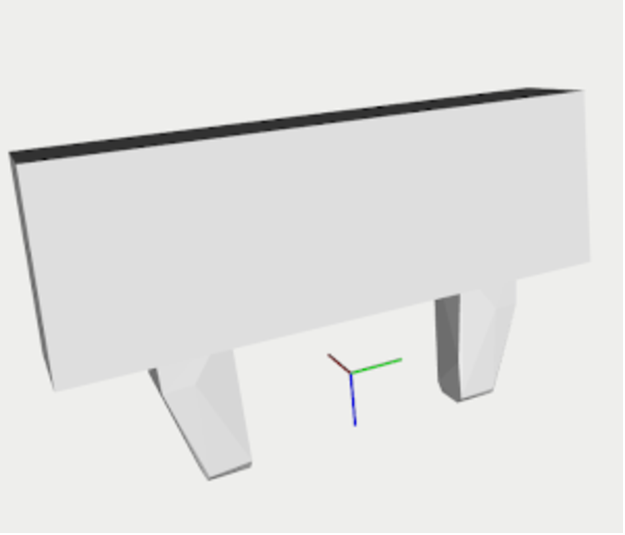
\includegraphics[width=\linewidth]{framework_manipulation/figures/hardware/mesh_cropped.pdf}
    \caption{Original mesh}\label{fig:original_mesh}
\end{subfigure}%
\hfill
\begin{subfigure}{0.3\columnwidth}
    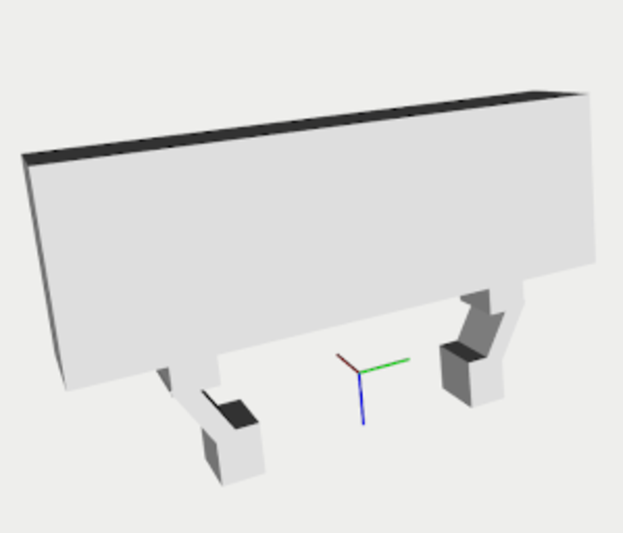
\includegraphics[width=\linewidth]{framework_manipulation/figures/hardware/doulbe_simple_cropped.pdf}
    \caption{Two fingers}\label{fig:two_fingers}
\end{subfigure}%
\hfill
\begin{subfigure}{0.3\columnwidth}
    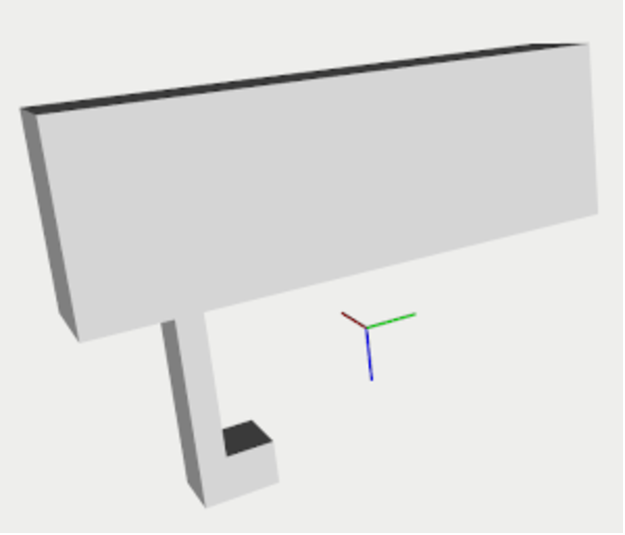
\includegraphics[width=\linewidth]{framework_manipulation/figures/hardware/single_hook_cropped.pdf}
    \caption{Hook finger}\label{fig:hook_finger}
\end{subfigure}

\caption{Original collision meshes are often approximated by convex hulls which are inaccurate while also more complex representations. In contrast, a simplified mesh can bring more accuracy as well as a computational performance gain in terms of simulation rate.}\label{fig:1}

\end{figure}

